% Format teze zasnovan je na paketu memoir
% http://tug.ctan.org/macros/latex/contrib/memoir/memman.pdf ili
% http://texdoc.net/texmf-dist/doc/latex/memoir/memman.pdf
% 
% Prilikom zadavanja klase memoir, navedenim opcijama se podešava 
% veličina slova (12pt) i jednostrano štampanje (oneside).
% Ove parametre možete menjati samo ako pravite nezvanične verzije
% mastera za privatnu upotrebu (na primer, u b5 varijanti ima smisla 
% smanjiti 
\documentclass[12pt,oneside]{memoir}

% Paket koji definiše sve specifičnosti mastera Matematičkog fakulteta
\usepackage[latinica]{matfmaster}
%
% Podrazumevano pismo je ćirilica.
%   Ako koristite pdflatex, a ne xetex, sav latinički tekst na srpskom jeziku
%   treba biti okružen sa \lat{...} ili \begin{latinica}...\end{latinica}.
%
% Opicija [latinica]:
%   ako želite da pišete latiniciom, dodajte opciju "latinica" tj.
%   prethodni paket uključite pomoću: \usepackage[latinica]{matfmaster}.
%   Ako koristite pdflatex, a ne xetex, sav ćirilički tekst treba biti
%   okružen sa \cir{...} ili \begin{cirilica}...\end{cirilica}.
%
% Opcija [biblatex]:
%   ako želite da koristite reference na više jezika i umesto paketa
%   bibtex da koristite BibLaTeX/Biber, dodajte opciju "biblatex" tj.
%   prethodni paket uključite pomoću: \usepackage[biblatex]{matfmaster}
%
% Opcija [b5paper]:
%   ako želite da napravite verziju teze u manjem (b5) formatu, navedite
%   opciju "b5paper", tj. prethodni paket uključite pomoću: 
%   \usepackage[b5paper]{matfmaster}. Tada ima smisla razmisliti o promeni
%   veličine slova (izmenom opcije 12pt na 11pt u \documentclass{memoir}).
%
% Naravno, opcije je moguće kombinovati.
% Npr. \usepackage[b5paper,biblatex]{matfmaster}

% Pomoćni paket koji generiše nasumičan tekst u kojem se javljaju sva slova
% azbuke (nema potrebe koristiti ovo u pravim disertacijama)
\usepackage{pangrami}

% Paket koji obezbeđuje ispravni prikaz ćiriličkih italik slova kada
% se koristi pdflatex. Zakomentarisati ako na sistemu koji koristite ovaj
% paket nije dostupan ili ako ne radi ispravno.
\usepackage{cmsrb}

% Ostali paketi koji se koriste u dokumentu
\usepackage{listings} % listing programskog koda

% Datoteka sa literaturom u BibTex tj. BibLaTeX/Biber formatu
\bib{matfmaster-primer}

% Ime kandidata na srpskom jeziku (u odabranom pismu)
\autor{Aleksandar Milosavljević}
% Naslov teze na srpskom jeziku (u odabranom pismu)
\naslov{Razvoj "Pure" okruženja za razvoj veb interfejsa}
% Godina u kojoj je teza predana komisiji
\godina{2021}
% Ime i afilijacija mentora (u odabranom pismu)
\mentor{dr Saša \textsc{Malkov}, vanredni profesor\\ Univerzitet u Beogradu, Matematički fakultet}
% Ime i afilijacija prvog člana komisije (u odabranom pismu)
\komisijaA{dr Aleksandar \textsc{Kartelj}, docent\\ Univerzitet u Beogradu, Matematički fakultet}
% Ime i afilijacija drugog člana komisije (u odabranom pismu)
\komisijaB{dr Ivan \textsc{Čukić}, docent\\ Univerzitet u Beogradu, Matematički fakultet}
% Ime i afilijacija trećeg člana komisije (opciono)
% \komisijaC{}
% Ime i afilijacija četvrtog člana komisije (opciono)
% \komisijaD{}
% Datum odbrane (obrisati ili iskomentarisati narednu liniju ako datum odbrane nije poznat)
\datumodbrane{15. јануар 2016.}

% Apstrakt na srpskom jeziku (u odabranom pismu)
\apstr{%
Rezime placeholder
}

% Ključne reči na srpskom jeziku (u odabranom pismu)
\kljucnereci{veb, internet, interfejs, html, css, javaskript, razvojno okruženje}

\begin{document}
% ==============================================================================
% Uvodni deo teze
\frontmatter
% ==============================================================================
% Naslovna strana
\naslovna
% Strana sa podacima o mentoru i članovima komisije
\komisija
% Strana sa posvetom (u odabranom pismu)
\posveta{Svima osim LaTex-u}
% Strana sa podacima o disertaciji na srpskom jeziku
\apstrakt
% Sadržaj teze
\tableofcontents*

% ==============================================================================
% Glavni deo teze
\mainmatter
% ==============================================================================

% ------------------------------------------------------------------------------
\chapter{Uvod}
Poboljšanje infrstrukture Internet mreže, to jest, povećanjem brzine i stabilnosti internet komunikacije,
naša interakcija sa računarima danas izgleda značajno drugačije nego pre 20 godina. Umesto stonih računara sa velikim kućištima i glasnim rashladnim sistemima,
današnji najrasprostranjeniji računari nam staju u džep. Koristimo ih kako bi komunicirali sa bližnjima i bili u toku sa svetskim dešavanjima.

Iako današnji mini računar koji gotovo svi nosimo u džepu ima više procesorske moći nego računar koji je korišćen tokom Appolo misije(ref), 
danas te lične računare ne koristimo za teška izračunavanja i komplikovane procedure. Koristimo ih najčešće kao terminale kako bismo pristupili internet resursima,
to jest, podacima koji se nalaze na velikim centralizovanim računarskim sistemima. Veb interfejs je tako postao glavni način naše interakcije sa računarom i internetom.

Posledica toga je značajna promena fokusa u svetu razvoja aplikativnog softvera. Ukoliko pogledamo rezultat upitnika kompanije "Stack Overflow" (ref)({\url{https://insights.stackoverflow.com/survey/2020#technology-programming-scripting-and-markup-languages-professional-developers}}) o najkorišćenijim programerskim alatima, videćemo da prva dva mesta na listi
zauzimaju upravo veb tehnologije (Na prvom mestu je JavaScript sa 69.7\%, dok je na drugom HTML/CSS sa 62.4\%).

Kako potreba za novim softverom daleko prevazilazi mogućnost softverskih inženjera da taj softver isporuče, biblioteke i okruženja koja pomažu pri razvoju softvera postali su veoma važan deo inženjerskog alata.
U domenu razvoja veb aplikacija, na tržištu se izdvajaju tri razvojna okruženja. Ova tri razvojna okruženja najviše se međusobno razlikuju po pristupu u promeni stanja aplikacije i razumevanju
toga šta je centralni deo dizajna (u funkcionalnom smislu) jedne veb aplikacije.

Kada posmatramo ova popularna razvojna okruženja, uočavamo dva bitno različita pristupa u arhitekturi:
\begin{enumerate}
  \item {\emph{Model-Pogled-Kontroler}} šablon u kom aplikacija predstavlja skup povezanih komponenti organizovanih u hijerarhisku strukturu, kojima je pridruženo stanje i ponašanje
  \item Flux šablon u kom se aplikacija posmatra kao mašina stanja čija je vizuelna reprezentacija samo rezultat trenutnog stanja.
\end{enumerate}

Prvi pristup je prisutan u okruženju Angular, drugi je dominantan u biblioteci React, dok Vue.js zastupa dizajn koji predstavlja kompromis izmеđu ova dva pristupa.

Kroz ovaj rad ispratićemo razvoj jednog modernog razvojnog okruženja za izradu SPA veb aplikacija.


% ------------------------------------------------------------------------------
\chapter{Arhitekture SPA aplikacija}
\section{Model-Pogled-Kontroler šablon}

\section{Flux šablon}
% ------------------------------------------------------------------------------
Razrada placeholder
% ------------------------------------------------------------------------------
\chapter{Problemi sa popularnim okruženjima}
\section{Upravljanje stanjem}
\section{Razdvajanje odgovornosti}
% ------------------------------------------------------------------------------
\chapter{Dizajn Pure okruženja}

Jedna od prvih odluka pri dizajniranju novog razvojnog okruženja,
jeste ta koje ćemo jezike i alate koristit pri samom pisanju okruženja.
Pri izboru jezika i alata važno je naći kompromisno rešenje između modernih
alata koji daju nove mogućnosti i
starih i u praksi oprobanih jezika i alata koji nude pouzdanost.

Jezik korišćen za pravljenje "Pure" razvojnog okruženja je TypeScript. TypeScript je
jezik razvijen od strane Microsoft-a kao alternativa JavaScript-u i zamišljen je kao njegov nadskup sa sistemom striktnih tipova podataka.
TypeScript je jezik koji se transpajlira na JavaScript korišćenjem TypeScript kompajlera.

Pošto je važno da proces prevođenja i testiranja razvoja što više automatizujemo i samim tim ubrzamo, neophodno je koristiti i "package bundler". 
Package bundler, pored toga što nam omogućava brže (manuelno) testiranje, koristi i tome da krajnjem korisniku razvojno okruženje isporučimo sa minifikovanim kodom.

Zbog minimalne potrebne konfiguracije Parcel je delovao kao odličan izbor.

\section{Dizajn elementi okruženja}
Jedna od specifičnijih stvari pri korišćenju React razvojnog okruženja jeste korišćenje JSX (ili TSX u Typescript verziji) jezika, koji objedinjuje JavaScript i HTML elemente u jednu
celinu i omogućava nam da html šablonima upravljamo kao objektima u JavaScript-u. Način na koji React ovo izvodi sastoji se u koraku transpilacije JSX fajla u JavaScript gde se svi elementi pisani html sintaksom prevode u čist JavaScript. 
Ovo, iako često može biti veoma korisna stvar, ponekad može da donese više problema nego rešava. Naime, iako kod koji koristimo za opisivanje vizuelne reprezentacije komponenata podseća na html,
on definitivno nije html, pa iz toga proizilaze ponekad čudne posledice. Na primer: ključnu reč 'class' ne možemo koristi u okviru JSX-template sintakse (zato što je 
'class' istovremeno rezervisana reč i u JavaScript-u i u HTML-u). Ovo je samo jedna dobro poznata "greška u dizajnu", dok su mnoge druge daleko prikrivenije i samim tim eventualne programerske greške koje mogu nastati pri transpilaciji mogu biti jako teške za otkrivanje.
Kako bi "Pure" framework zadržao mogućnost upravljanja komponenatama nivoa pogleda kao regularnim JavaScript objektima, a istovremeno izbegao eventualne komplikacije koje uvode jezici kao što je to JSX, kao deo Pure razvojnog okruženja napisana je biblioteka za opis sloja pogleda komponente.
\section{Biblioteka dom elemenata}
Biblioteka dom elemenata zamišljena je kao zamena za template engine
\section{Reaktivno programiranje}
\section{Optimizacije}

\chapter{Primer kroz TODO aplikaciju}
\chapter{Primeri korišćenja}
% ------------------------------------------------------------------------------
% \section{Примери коришћења класичних \LaTeX{} елемената}
% % primeri citiranja
% Ово је реченица у којој се јавља цитат \cite{PetrovicMikic2015}.
% Још један цитат \cite{GuSh:243}.
% % primeri navodnika
% Испробавамо наводнике: "Рекао је да му се јавимо сутра".
% % primer referisanja na tabelu (koja se javlja kasnije)
% У табели \ref{tbl:rezultati} која следи приказани су резултати експеримента.
% % primer kraćeg latiničkog teksta
% Ovo je primer rečenice ispisane latiničkim pismom u okviru ćiriličkog dokumenta.
% У овој реченици се налази једна {\lat reč} написана латиницом.
% % primer korišćenja fusnota
% Иза ове реченице следи фуснота.\footnote{Ово је фуснота.}
% % primer url-a
% Сајт математичког факултета је \url{http://www.matf.bg.ac.rs}.

% % primer dužeg latiničkog teksta
% \begin{latinica}
%   Ovo je malo duži blok teksta ispisan latiničkim pismom u okviru
%   ćiriličkog dokumenta. Fijuče vetar u šiblju, ledi pasaže i kuće iza
%   njih i gunđa u odžacima.
% \end{latinica}

% % primer korišćenja tabele
% \begin{table}
% \centering
% \caption{Резултати}
% \label{tbl:rezultati}
% \begin{tabular}{c>{\centering}p{2cm}c}
% \toprule
% 1 & 2 & 3\\\midrule
% 4 & 5 & 6\\\cmidrule(rl){1-2}
% 7 & 8 & 8\\
% \bottomrule
% \end{tabular}
% \end{table}

% % primer korišćenja slike
% \begin{figure}[!ht]
%   \centering
%   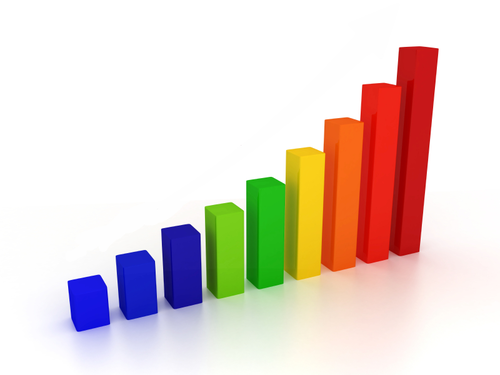
\includegraphics[width=0.5\textwidth]{graph.png}
%   \caption{Графикон}
%   \label{fig:grafikon}
% \end{figure}

% % primer jednostavnije matematičke formule
% Ево и један пример математичке формуле: $e^{i\pi} + 1 = 0$. 
% % primer referisanja na sliku
% На слици \ref{fig:grafikon} приказан је један графикон.

% % primer kompleksnije matematičke formule
% $$
% \int_a^b f(x)\ \mathrm{d}x \ =_{def}\ \lim_{\max{\Delta x_k \rightarrow 0}} \sum_{k=1}^n f(x_k^*)\Delta x_k
% $$

% % primer referisanja na poglavlja i strane poglavlja
% Више детаља биће дато у глави \ref{chp:razrada} на страни \pageref{chp:razrada}.

% % primer listinga koda

% У тезу можемо убацити и програмски кôд.

% \begin{verbatim}
% Ovo je doslovni tekst.
% \end{verbatim}

% % \begin{english}
% \lstset{
%   language=C,
%   basicstyle=\ttfamily,
%   keywordstyle=\color{blue}
% }
% \begin{lstlisting}
% #include <stdio.h>

% int main() {
%    printf("Hello, world!\n");
%    return 0;
% }
% \end{lstlisting}
% % \end{english}


Овај C програм се може превести помоћу преводиоца GCC \cite{gcc}.

% % primer liste
% Можемо правити и набрајања:
% \begin{enumerate}
% \item Анализа 1
% \item Линеарна алгебра
% \item Аналитичка геометрија
% \item Основи програмирања
% \end{enumerate}



% ------------------------------------------------------------------------------
% Literatura
% ------------------------------------------------------------------------------
\literatura

% ==============================================================================
% Završni deo teze i prilozi
\backmatter
% ==============================================================================

% ------------------------------------------------------------------------------
% Biografija kandidata
\begin{biografija}
\textbf{Вук Стефановић Караџић} (\emph{Тршић, 26. октобар/6. новембар
  1787. — Беч, 7. фебруар 1864.}) био је српски филолог, реформатор
српског језика, сакупљач народних умотворина и писац првог речника
српског језика.  Вук је најзначајнија личност српске књижевности прве
половине XIX века. Стекао је и неколико почасних доктората.
Учествовао је у Првом српском устанку као писар и чиновник у
Неготинској крајини, а након слома устанка преселио се у Беч,
1813. године. Ту је упознао Јернеја Копитара, цензора словенских
књига, на чији је подстицај кренуо у прикупљање српских народних
песама, реформу ћирилице и борбу за увођење народног језика у српску
књижевност. Вуковим реформама у српски језик је уведен фонетски
правопис, а српски језик је потиснуо славеносрпски језик који је у то
време био језик образованих људи. Тако се као најважније године Вукове
реформе истичу 1818., 1836., 1839., 1847. и 1852.
\end{biografija}
% ------------------------------------------------------------------------------

\end{document} 